% !TEX encoding = UTF-8 Unicode

\chapter{Podsumowanie}

Zwieńczeniem całej pracy i stworzonych modeli są dwa skrypty rozpoznające ilość
oczek wyrzuconych na kości w czasie rzeczywistym. Programy korzystają z wytrenowanych
modeli załadowanych do pamięci, które analizują obraz dostarczany z kamery
podłączonej do komputera. Modele są przystosowane do rozpoznawania kości na
obrazach o wielkościach 64x64 oraz 106x79 pikseli.\\
Obraz 1600x1200 dostarczany z kamery jest wielokrotnie większy, co wymusiło wyznaczenie jego
części, która jest analizowana przez zaaplikowane sieci neuronowe. Ta część obrazu została
oznaczona białymi krawędziami dla łatwiejszego zlokalizowania miejsca, w którym
powinna być umieszczona kość pod kamerą (zob. rys. \ref{fig:recognize}) :\\
\begin{figure}[h!]
\begin{center}
\begin{tabular}{cc}
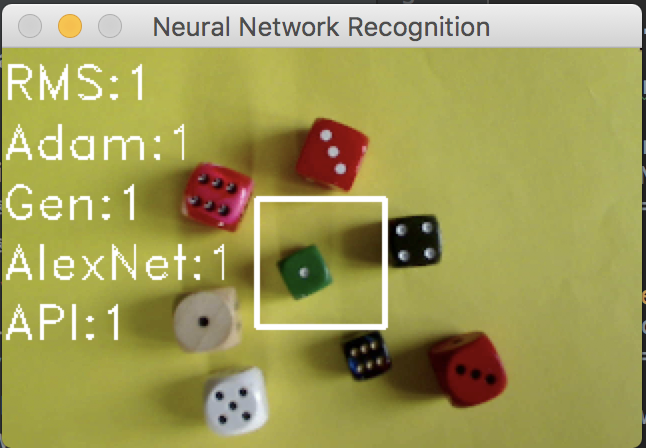
\includegraphics[width=0.49\linewidth]{neural_network_recognition} &
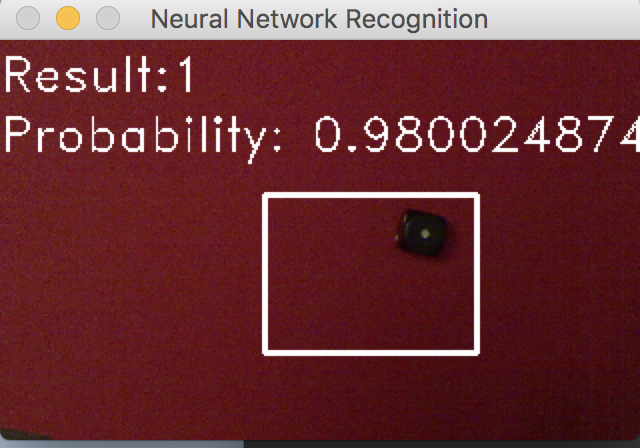
\includegraphics[width=0.49\linewidth]{neural_network_recognition_106x79} \\
Rozpoznawanie obrazów 64x64 & Rozpoznawanie obrazów 106x79\\
\end{tabular}
\captionof{figure}{Przykłady działania sieci neuronowych}
\label{fig:recognize}
\end{center}
\end{figure}\\
Dla obrazów 64x64 wykonano kilka modeli sieci, które osiągnęły powyżej 90\% skuteczności.
Program umożliwia porównanie wyników dzięki zaaplikowaniu ich do analizy tego
samego obszaru na zdjęciu. Pozwala to zauważyć między innymi lepsze rozpoznawanie
pewnych kombinacji kolorystycznych niektórych modeli lub trudności z rozróżnieniem
wyrzuconych czterech oczek od sześciu, z uwagi na efekt zlewania się ich podczas
skalowania.\\
Dla obrazów 106x79 zaaplikowany jest jedynie jeden model, wytrenowany przez 100 epok.\\
Wyniki zaobserwowane podczas prac związanych z tworzeniem sieci neuronowych przyniosły
wiele niespodziewanych sytuacji. Wielokrotnie otrzymywane wyniki były zdumiewające,
biorąc pod uwagę, jak drobne różnice w budowie sieci wpływały na końcowe rezultaty.\\
Wszystkie eksperymenty pokazały, że nawet proste zadanie rozpoznawania oczek na kostce
wymaga dużej ilości danych i mocy obliczeniowej, by uzyskać satysfakcjonujące wyniki.
Przykład ten pokazuje także jak wiele zastosowań może mieć zyskujące na popularności
uczenie maszynowe, które wraz z rozwojem technologii będzie mieć coraz więcej możliwości
na dostosowywania algorytmów do określonych danych.
